\chapter{\label{chap:related-work}Trabalhos Relacionados}
% MarI/O
% - https://www.youtube.com/watch?v=qv6UVOQ0F44 
% - https://www.youtube.com/watch?v=iakFfOmanJU 
% - https://www.youtube.com/watch?v=S9Y_I9vY8Qw 

% Atari DeepMind
% - http://arxiv.org/pdf/1312.5602v1.pdf 
% - https://storage.googleapis.com/deepmind-data/assets/papers/DeepMindNature14236Paper.pdf  

% NERO
% - http://nn.cs.utexas.edu/?stanley:ieeetec05 

\section{N.E.R.O: Neuro-Evolving Robotic Operatives}

\begin{mdframed}[backgroundcolor=green!20]
\begin{itemize}
    \item
        O que é
    \item
        Técnica utilizada (citar paper)
    \item
        Relevância com o nosso trabalho
\end{itemize}
\end{mdframed}

%----------
\section{Atari DeepMind}

\begin{mdframed}[backgroundcolor=green!20]
\begin{itemize}
    \item
        O que é
    \item
        Técnica utilizada (citar paper)
    \item
        Relevância com o nosso trabalho
\end{itemize}
\end{mdframed}

%----------
\section{MarI/O}

Em junho de 2015, o canal do \textit{YouTube}
SethBling\footnote{https://www.youtube.com/user/sethbling/about} -- conhecido
por publicar vídeos de modificações de jogos como Mario e Minecraft -- publicou
o vídeo \textit{MarI/O - Machine Learning for Video
Games}\footnote{https://www.youtube.com/watch?v=qv6UVOQ0F44}, que mostra um
jogador muito habilidoso jogando o jogo \textit{Super Mario World}. É explicado
então que o jogador em questão não é um jogador humano, mas sim um programa de
computador.
O vídeo mostra que é feito o uso de uma técnica chamada
\textit{\textbf{NEAT}} (\textit{NeuroEvolution of Augmenting
Topologies})\cite{stanley:ec02}, que consiste em utilizar algoritmos
genéticos e redes neurais para poder construir uma inteligência artificial
que melhore o seu desempenho à medida que explora mais situações do jogo. A
técnica \textit{NEAT} é explicada de forma mais detalhada no capítulo
\ref{chap:neat}. Combinada com a linguagem de programação \textit{Lua}, a
técnica é então usada para construir um jogador que é capaz de ir do início ao
fim de uma fase de \textit{Super Mario World} com sucesso.

\begin{figure}[htb!]
\centering
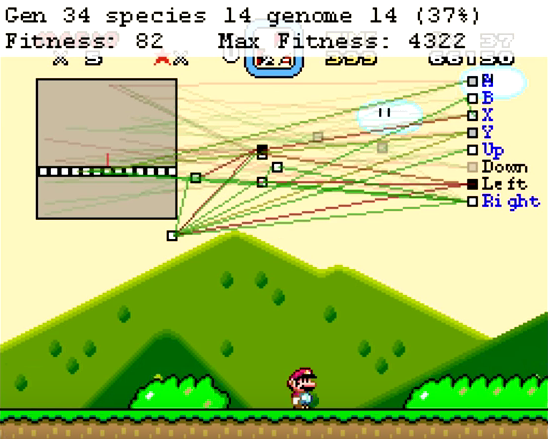
\includegraphics[width=.65\textwidth]{fig/mar-io-example.png}
\caption{\label{fig:mar-io-example}Exemplo da visão do jogo \textit{Super
Mario World} através do projeto \textit{MarI/O}, mostrando elementos de
controle usados pelo NEAT, como a rede neural, as possíveis ações, as
gerações, especies, genomas e outros.}
\end{figure}

O \textit{MarI/O} é especialmente interessante e relevante para este trabalho
pois traz à tona o uso da técnica \textit{NEAT} para a criação de uma
inteligência artificial capaz de jogar uma partida de um jogo, sendo este
um dos objetivos desse trabalho. O que temos de diferente, e que trate-se de um
desafio a mais, é o fato de que no caso do Spelunky, os níveis, além de serem
gerados proceduralmente, são dispostos em 16 salas (explicado na seção
\ref{section:spelunky-procgen}), fazendo com que seja mais difícil de
medir o quão melhor um jogador é quando comparado à outro. Principalmente
pois não sabemos o quão perto estamos da saída da caverna sem encontrá-la
primeiro.
